\documentclass[10pt,a4paper]{article}
\usepackage[utf8]{inputenc}
\usepackage{amsmath}
\usepackage{amsfonts}
\usepackage{amssymb}
\usepackage{listings}
\usepackage{xcolor}
\usepackage{svg}

\author{Maximilian Prietzel}
\title{Abiturvorbereitung Informatik}

\begin{document}

\maketitle
\tableofcontents
\newpage


\section{1. Semester}

\subsection{Datenstrukturen}
\subsubsection{Listen}



\subsection{Objektorientierung}
\lstset{
	language=java, 				% Setzt die Sprache
	basicstyle=\scriptsize\ttfamily, 	% Setzt den Standardstil
	keywordstyle=\color{violet} \bfseries,	% Setzt den Stil für Schlüsselwörter
	identifierstyle=\color{brown},		% Identifier bekommen keine gesonderte formatierung
	commentstyle=\color{gray},		% Stil für Kommentare
	stringstyle=\color{teal}, 			% Stil für Strings (gekennzeichnet mit "String")
	breaklines=true, 			% Zeilen werden umgebrochen
	numbers=left, 				% Zeilennummern links
	numberstyle=\tiny, 			% Stil für die Seitennummern
	frame=single, 				% Rahmen
	%backgroundcolor=\color{black}, 	% Hintergrundfarbe
	%caption={Javaklasse}, 			% Caption
	tabsize=2				% Größe der Tabulatoren
}
\subsubsection{Klasse/Objekt}
Eine Klasse ist wie der Bauplan eines Objektes, sie beinhaltet die Informationen, welche Attribute und Methoden das Objekt besitzt. \\
Beispiel Java: 
\begin{lstlisting}
public class Katze
{
  //Attribute
  static private int beine = 4;  //static variable
  private String name;
  private int alter;

  //Konstruktor
  Katze(int name, int alter)
  {
    this.name = name;
    this.alter = alter;
  }

  //Methoden
  public void miau()
  {
    System.out.println("Miau");
  }

  public String getName()
  {
    return name;
  }
}
\end{lstlisting} 
Das Objekt kann mithilfe der Instanzisierung in einer Variable (Instanz) gespeichert werden.\\
\\
Ein Objekt wird mithilfe des Konstruktors erstellt. \\
So würde in Java ein Objekt erstellt werden: 
\begin{lstlisting}
class  Programm 
{  
    public static void main(String args[])  //main method  
    {  
       Katze garfield = new Katze("Garfield" ,  10);
       garfield.miau(); //Output: Miau
    }  
}  
\end{lstlisting}
Die Schlüsselwörter \textcolor{violet}{public} und  \textcolor{violet}{private} bestimmen wann und ob ein anderes Objekt auf diese Variable/Methode zugreifen kann. \\
\\
\begin{tabular}{c|c}
\textcolor{violet}{public}   & Jeder kann darauf zugreifen\\
\hline
\textcolor{violet}{private} & Nur die eigene Klasse kann darauf zugreifen\\
\hline
\textcolor{violet}{protected}* & Die Subklasse kann darauf zugreifen  \\
\hline
\textcolor{violet}{package private}* & Das eigene Paket kann darauf zugreifen\\
\end{tabular}
\newpage

\subsubsection{UML-Klassendiagramm}
\begin{tabular}{c|c|c}

\includegraphics[width=1cm]{kompostion.png}   & Kompostion & \\
\hline

\includegraphics[width=1cm]{aggregation.png}  &Aggregation &\\
\hline

\includegraphics[width=1cm]{asso.png}  &Assoziation &  \\
\hline

\includegraphics[width=1cm]{vererbung.png}  & Vererbung &\\
\end{tabular}
\\ \\ \\
\underline{Beispiel UML-Diagramm:} \\
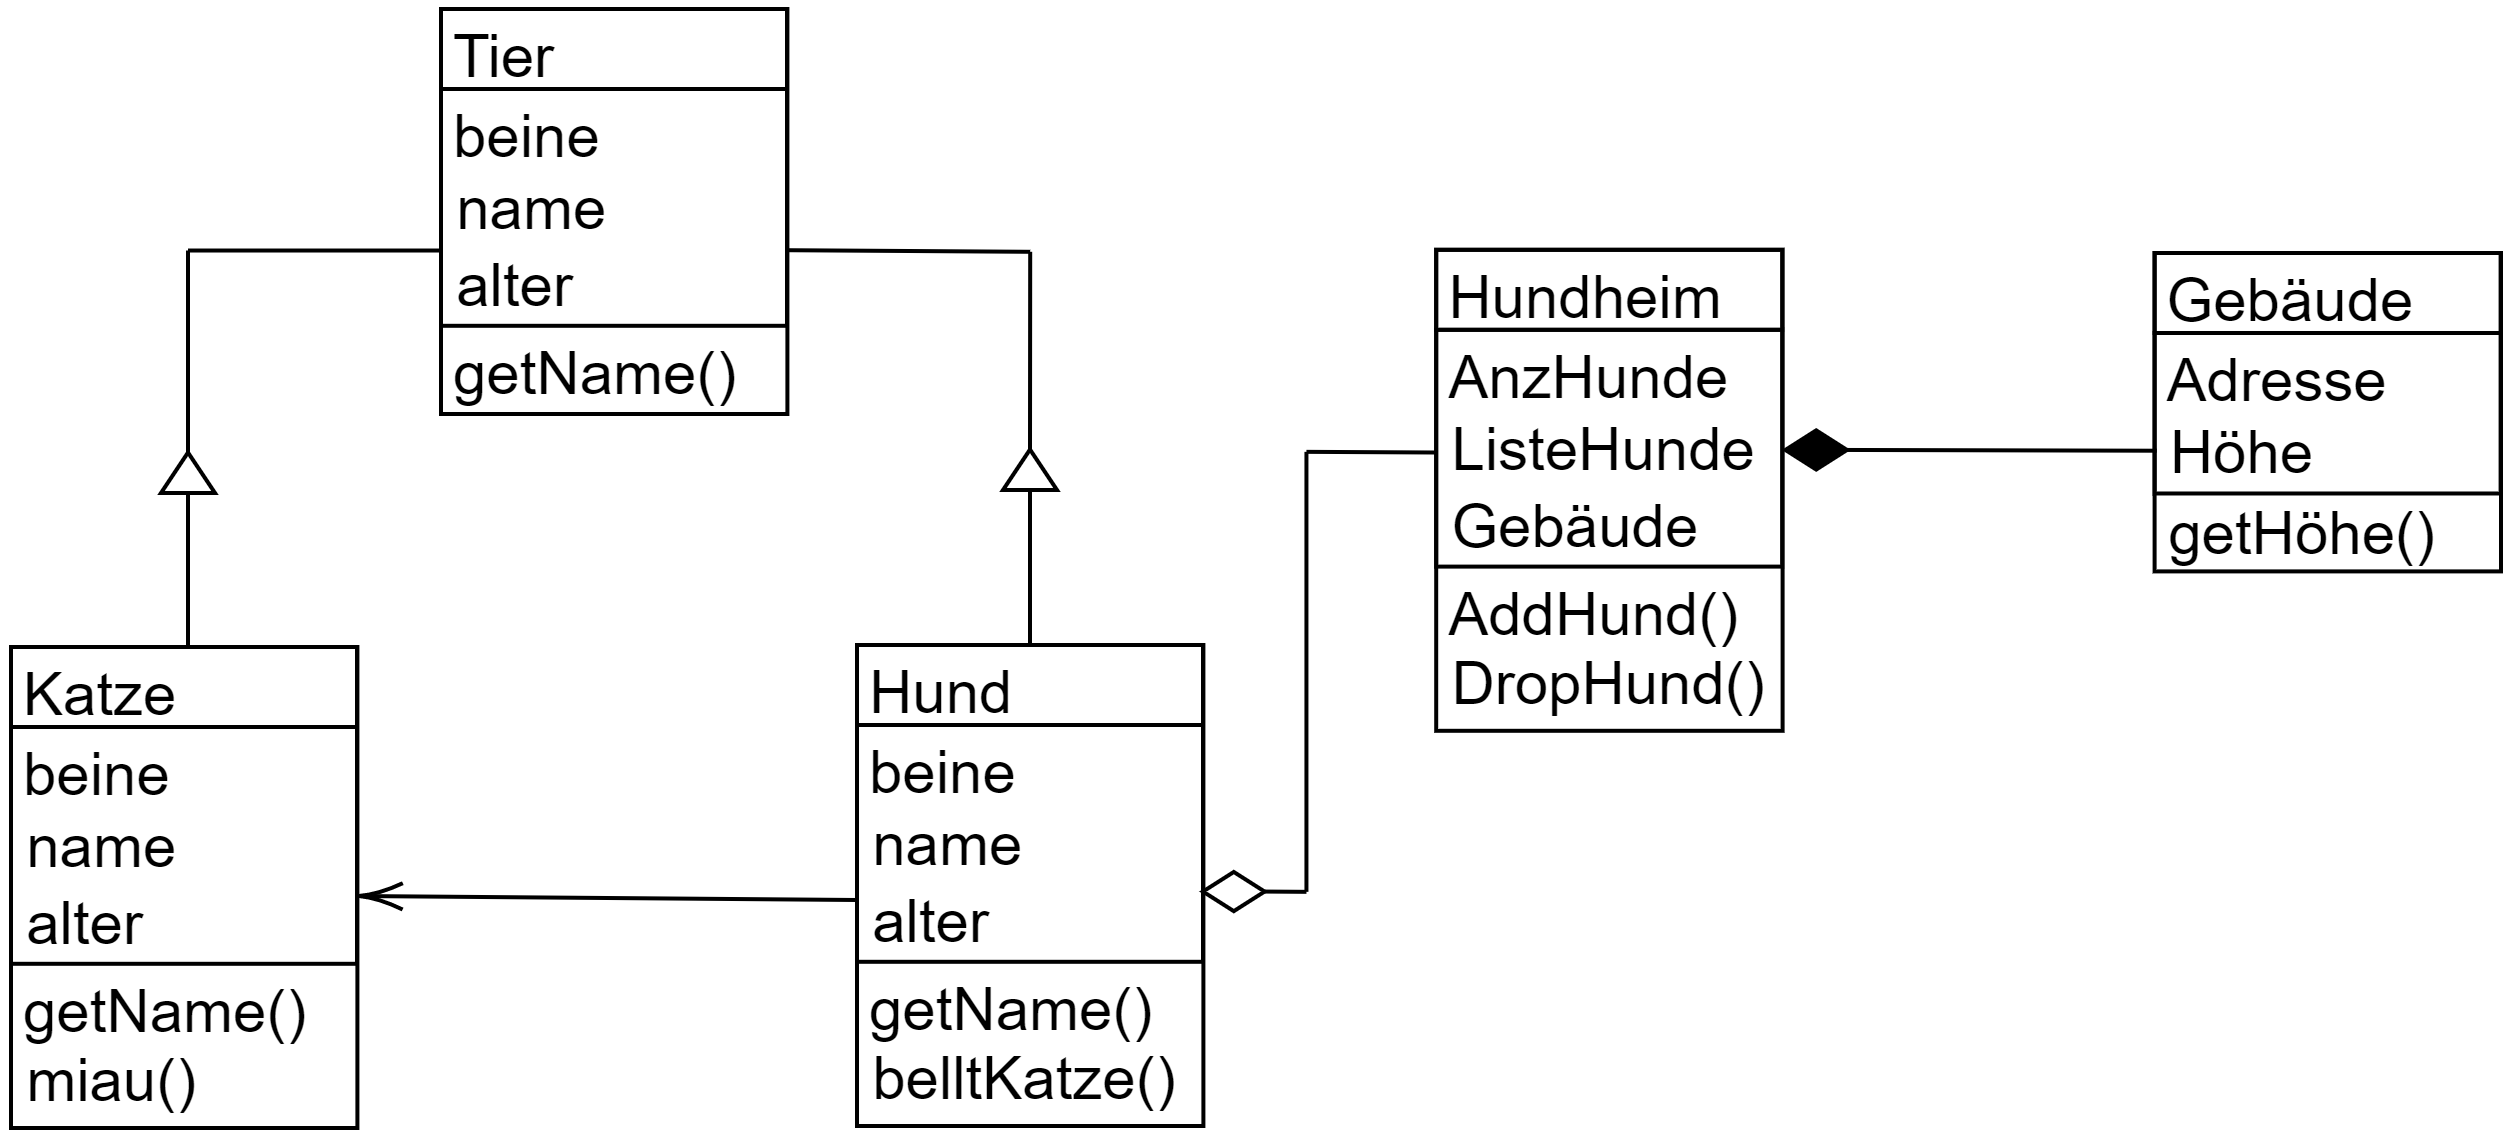
\includegraphics[width=10cm]{uml.png} 

\newpage

\section{2. Semester}

\subsection{Mengenlehre}
\subsubsection{Mengenoperationen}
\begin{tabular}{c|c|c}
Symbol & Name & SQL-Befehl \\
\hline
$\cup$ & Vereinigungsmenge & \textcolor{blue}{UNION} \\
\hline
$\cap$ & Schnittmenge & \textcolor{blue}{INTERSECT} \\
\hline
$\backslash$ & Differenzmenge & \textcolor{blue}{EXCEPT} \\
\hline
$A \times B$ & Kartesisches Produkt & \textcolor{blue}{SELECT} * \textcolor{blue}{FROM} A,B\\
\hline
$\subseteq$ & Teilmenge &  \\
\hline
$\subset$ & Echte Teilmenge &  \\
\end{tabular}
\subsubsection{Venn-Diagramme}

\subsection{Datenbankentwurf}

\newpage

\section{3. Semester}

\subsection{Theoretische Informatik}
\subsection{Netzwerke}

\subsection{Netzwerktopologie}


\end{document}